
\newglossaryentry{V-Modell 97}
{
    singular={V-Modell 97},
    plural={V-Modell 97},
    name={V-Modell 97},
    description={
        Eine Weiterentwicklung des \textbf{V-Modell nach Boehm} und empfohlenes Vorgehensmodell bei Softwareprojekten, die im Auftrag der BRD umgesetzt werden.\\
        Basiert auf 4 Submodellen: \textit{Projektmanagement}, \textit{Qualitätssicherung}, \textit{Systemerstellung}, \textit{Konfigurationsmanagement}\footnote{s. a. \url{https://t2informatik.de/wissen-kompakt/v-modell-97/}, abgerufen 26.03.2024)}
        2005 abgelöst durch \textbf{V-Modell XT}.
    }
}

\newglossaryentry{V-Modell nach Boehm}
{
    singular={V-Modell nach Boehm},
    plural={V-Modell nach Boehm},
    name={V-Modell nach Boehm},
    description={
        Vorgehensmodell bzw. Prozessreferenzmodell für die Softwareentwicklung (als \textit{Wasserfallmodell}), vorgeschlagen 1979 durch \textit{Barry Boehm}.
        \begin{figure}
            \centering
            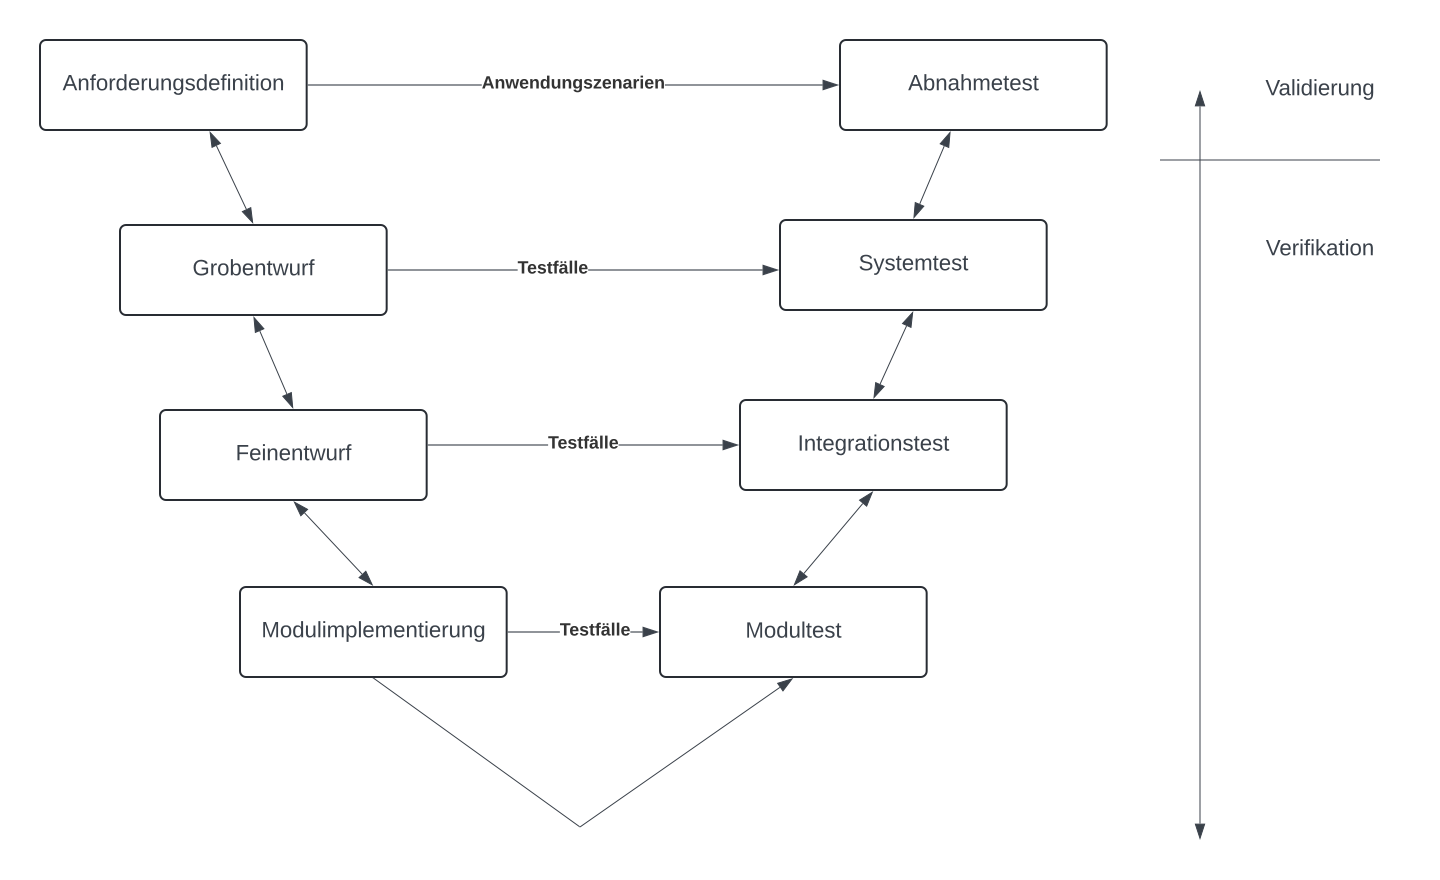
\includegraphics[scale=0.3]{chapters/Glossar/img/vmodell}
            \caption{Das Vorgehensmodell nach Boehm. (Quelle: in Anlehnung an \cite[554, Abb. 20.11-2]{Bal08})}
        \end{figure}
    }
}

\newglossaryentry{V-Modell XT}
{
    singular={V-Modell XT},
    plural={V-Modell XT},
    name={V-Modell XT},
    description={
        Weiterentwicklung des \textit{V-Modell 97}. Basiert auf aufeinander
        aufbauenden Vorgehensbausteinen, die die modularen EInheiten des
        V-Modells bilden. Verpflichtende Vorgehensbausteine als Kern des Modells
        betreffen das Projektmanagement, die Qualitätssicherung, das Konfigurations-,
        Problem und Änderungsmanagement, die allesamt ein Mindestmaß von Projektdurchführungsqualität
        gewährleisten sollen. Das V-Modell XT ist mit 18 Vorgehensbausteinen
        weitaus feingranularer konzeptioniert, wodurch es leichter an Projektspezifika
        anzupassen ist (``\textit{Tailoring}``) als das V-Modell 97 (vgl.~\cite[329 f.]{AABG14n})
    }
}

\newglossaryentry{Tailoring}
{
    singular={Tailoring},
    plural={Tailoring},
    name={Tailoring},
    description={
        Projektspezifische Anpassung eines Phasenmodells an die konkrete Projektaufgabe  (vgl.~\cite[330]{AABG14n})
    }
}

\newglossaryentry{Team Software Process (TSP)}
{
    singular={Team Software Process (TSP)},
    plural={Team Software Process (TSP)},
    name={Team Software Process (TSP)},
    description={
        Der Team Software Prozess (TSP) ist eine Methode für Softwareentwicklungsteams zur Selbstoptimierung.
        [...]
        Durch die Verwendung von TSP sollen folgende Ziele erreicht werden:
        \begin{itemize}
            \item Bessere und genauere Planung (dadurch bessere Erfüllung von geplanten Daten)
            \item Verbesserung der Qualität des Produktes
            \item Niedrigere Kosten von Projekten (Total Cost of Ownership)}\footnote{
Quelle: \url{https://de.wikipedia.org/wiki/Team_Software_Process}, abgerufen 26.03.2024
}
        \end{itemize}
    }
}

\newglossaryentry{DV-Konzept}
{
singular={DV-Konzept},
plural={DV-Konzept},
name={DV-Konzept},
description={
\textit{Datenverarbeitungskonzept}. Relevante Daten werden von dem Fachkonzept in ein Modell (Persistierung / Verarbeitung) für eine konkrete Datenbank und/ oder Programmiersprache überführt. Im Wasserfallmodell ist das die Fortführung des \textit{Fachkonzeptes} (aus der 2. Phase ``\textit{Analyse}``) in der dritten Phase ``\textit{Entwurf}``.
}
}

\newglossaryentry{Requirements Engineering}
{
singular={Requirements Engineering},
plural={Requirements Engineering},
name={Requirements Engineering},
description={
Systematisches Vorgehen des Ermittelns von Anforderungen für ein (Software-)Produkt.
}
}

\newglossaryentry{Kunde}
{
singular={Kunde},
plural={Kunde},
name={Kunde},
description={
Beauftragt die Software, investiert in die Umsetzung und verspricht sich einen (wirtschaftlichen) Nutzen davon.
Muss nicht zwingend auch \textbf{Anwender} der Software sein.
}
}


\newglossaryentry{Anwender}
{
singular={Anwender},
plural={Anwender},
name={Anwender},
description={
Arbeitet mit der Software, bspw. als Endanwender oder Administrator, der für Betrieb und Installation auf den Rechnern zuständig ist.
Kann ein Mitarbeiter des \textbf{Kunden} sein, kann aber auch nicht greifbarer Endanwender auf dem \textit{anonymen Markt} sein.
}
}


\newglossaryentry{Domäne}
{
singular={Domäne},
plural={Domäne},
name={Domäne},
description={
\textbf{Domäne} oder auch \textbf{Anwendungsdomäne} bezeichnet das (abgegrenzte) fachliche Umfeld, für das die Software entwickelt werden soll (vgl.~\cite[41]{Wed09})
}
}

\newglossaryentry{Domänenanalyse}
{
singular={Domänenanalyse},
plural={Domänenanalyse},
name={Domänenanalyse},
description={
Prozess, in dem Entwickler Hintergrundinformationen zu der Aufgabe und das Umfeld suchen, systematisch analysieren und sich (dabei) Wissen über die Fachlichkeit aneignen.
}
}


\newglossaryentry{Requirements}
{
singular={Requirements},
plural={Requirements},
name={Requirements},
description={
\textbf{Requirements} oder auch \textbf{Anforderungen} sind die funktionalen und nicht-funktionalen Anforderungen, die aus Sicht der Anwender für die Software wichtig sind  (vgl.~\cite[41]{Wed09})
}
}

\newglossaryentry{Business Case}
{
singular={Business Case},
plural={Business Case},
name={Business Case},
description={
``Ein Business Case ist ein Szenario zur betriebswirtschaftlichen Beurteilung einer Investition.`` (\cite[11]{Brug09})
}
}

\newglossaryentry{Projektbeteiligte}
{
singular={Projektbeteiligte},
plural={Projektbeteiligte},
name={Projektbeteiligte},
description={
s. \textbf{Stakeholder}
}
}

\newglossaryentry{Pseudozustand}
{
singular={Pseudozustand},
plural={Pseudozustand},
name={Pseudozustand},
description={
In einem \textbf{Zustandsautomaten} (UML) ist ein \textbf{Pseudozustand} ein Zustand, mit dessen Hilfe eine bestimmte Ablauflogik modelliert werden kann, wie \textit{Balzert} in \cite[542]{Bal05} erklärt. Hierzu gehören
\begin{itemize}
\item Anfangszustand
\item Entscheidungszustand
\item Kreuzung
\item Terminator
\item Historie
\item Eintritts- und Austrittspunkt
\end{itemize}
}
}




\newglossaryentry{Stakeholder}
{
singular={Stakeholder},
plural={Stakeholder},
name={Stakeholder},
description={
Unter \textbf{Stakeholder} (\textit{Projektbeteiligte}) werden nach DIN 69901-5 im Projektmanagement die Projektteilnehmenden,
Projektbetroffenen und Projektinteressierten verstanden.
Auch Endanwender gehören zu den Stakeholdern.
\textit{Wedemann} faßt \textbf{Stakeholder} wie folgt zusammen: ``Personen, Gruppen oder Organisationen, die aktiv am Projekt beteiligt sind, von deren Auswirkungen betroffen sind oder die Möglichkeit haben, das Projekt zu beeinflussen.`` (\cite[49]{Wed09})\\
}
}


\newglossaryentry{Geschäftsanforderungen}
{
singular={Geschäftsanforderungen},
plural={Geschäftsanforderungen},
name={Geschäftsanforderungen},
description={
Anforderungen, die aus einer Geschäftsidee folgen, und die beschreiben, ein Projekt zu einem kommerziellen Erfolg wird. I.d.R. ein Produkt des \textbf{Vision \& Scope} sowie Bestandteil des \textbf{Business Case}
}
}
\newglossaryentry{Lastenheft}
{
singular={Lastenheft},
plural={Lastenheft},
name={Lastenheft},
description={
siehe \textbf{Vision \& Scope}
}
}


\newglossaryentry{Vision and Scope}
{
singular={Vision and Scope},
plural={Vision and Scope},
name={Vision and Scope},
description={
Auch \textbf{Lastenheft}: Dokument, in dem die Ziele des Kunde und der Projektumfang dokumentiert wird. Enthält die Anforderungen an das Produkt, damit es für den Kunden ein Erfolg wird.\\
\blockquote[{\cite[305]{AABG14m}}]{
Das Lastenheft wird vom Auftraggeber (AG) erarbeitet und hat
nach DIN 69905 die Gesamtheit der Forderungen an die Lieferungen und Leistungen eines Auftragnehmers zum Inhalt. Der Zweck eines Lastenhefts ist die Einholung von Angeboten von potentiellen Auftragnehmern. Das Lastenheft beschreibt
in der Regel also, was und wofür etwas gemacht werden soll. Der Adressat des
Lastenhefts ist der (externe oder interne) Auftragnehmer.
}


}
}


\newglossaryentry{Phasenmodell}
{
singular={Phasenmodell},
plural={Phasenmodell},
name={Phasenmodell},
description={
``Ein \textit{Vorgehensmodell} oder auch \textit{Phasenmodell} beschreibt die Systementwicklung
eines IS [Informationssystems] in Form von Aktivitäten. Diese Aktivitäten sind den unterschiedlichen
Phasen zugeordnet. Es wird festgelegt, in welcher Reihenfolge die Aktivitäten
durchgeführt werden können und welche Überschneidungen zulässig sind.`` (\cite[316]{AABG14n})
}
}

\newglossaryentry{Prozessmodell}
{
singular={Prozessmodell},
plural={Prozessmodell},
name={Prozessmodell},
description={
``Allgemeiner Entwicklungsplan, der das generelle Vorgehen beim Entwickeln eines Produkts festlegt.`` (\cite[694]{Bal08})
}
}

\newglossaryentry{Evolutionäres Modell}
{
singular={Evolutionäres Modell},
plural={Evolutionäres Modell},
name={Evolutionäres Modell},
description={
Vorgehensmodell, bei dem ein Produktkern (\textit{Nullversion}) entwickelt wird, anhand dessen der Auftraggeber weitere Anforderungen ermittelt. (vgl.\cite[529 f.]{Bal08})
}
}

\newglossaryentry{Entwurf}
{
singular={Entwurf},
plural={Entwurf},
name={Entwurf},
description={
Aus der \textbf{Entwurfsphase} geht der \textbf{Entwurf} hervor, der die Aufgabe hat, aus den Ergebnissen der \textbf{OOA} eine Anwendung unter den geforderten technischen Randbedingungen zu realisieren. Hierbei wird das \textbf{OOD}-Modell unter den Gesichtspunkten \textit{Standardisierung} und \textit{Effizienz} konzipiert (vgl.~\cite[13]{Bal05}).
}
}

\newglossaryentry{Pflichtenheft}
{
singular={Pflichtenheft},
plural={Pflichtenheft},
name={Pflichtenheft},
description={
Nachdem vom AG das \textbf{Lastenheft} erstellt wurde, erstellt der AN das \textbf{Pflichtenheft}:
\blockquote[{\cite[306]{AABG14m}}]{
Das Pflichtenheft ist nach DIN 69905 die Beschreibung der vom Auftragnehmer erarbeiteten Realisierungsvorgaben. Es sollte das vom Auftraggeber vorgegebene
Lastenheft umsetzen. Es wird als Teil eines Angebots vom Auftragnehmer erstellt.
Das Pflichtenheft enthält eine Zusammenfassung aller fachlichen Anforderungen,
die das zu entwickelnde Produkt/Dienstleistung aus der Sicht des Auftragnehmers
erfüllen muss. Dabei geht es um den Funktions-, Leistungs- und Qualitätsumfang
des Produkts. Das Pflichtenheft muss so abgefasst sein, dass es als Basis eines juristischen Vertrags dienen kann.
}
\noindent
Das Pflichtenheft dient dem \textit{Systemanalytiker} als Grundlage zur Erstellung des \textbf{OOA-Modells}.
}
}

\newglossaryentry{Anwendungsfall}
{
singular={Anwendungsfall},
plural={Anwendungsfall},
name={Anwendungsfall},
description={
``Ein \textbf{Anwendungsfall} beschreibt anhand eines zusammenhängenden Arbeitsablaufes die Interaktionen mit einem (geschäftlichen oder technischen) System. Ein Anwendungsfall wird stets durch einen Akteur initiiert und führt gewöhnlich zu einem für die Akteure wahrnehmbaren Ereignis.`` (\cite[351]{Oes05})
}
}

\newglossaryentry{Aktive Redundanz}
{
singular={Aktive Redundanz},
plural={Aktive Redundanz},
name={Aktive Redundanz},
description={
\textbf{Aktive Redundanz} ist eine Taktik zur Verhinderung von Fehlfunktionen als Teil der Planung einer Softwarearchitektur: Redundante Systeme bearbeiten Anfragen gleichzeitig. Die Antwort des schnellsten Systems wird verwendet (s. \textit{Functional redundancy}, \cite[90]{BCK12}).
}
}

\newglossaryentry{MOF}
{
singular={MOF},
plural={MOF},
name={MOF},
description={
\textbf{MOF} (\textit{Meta Object Facility}) ist Grundlage für die Definitionen des UML-Metamodells. Die Metaebene der MOF wird auch \textbf{M3} bezeichnet. Das Metamodell der UML 2.0 ist auch Ebene \textbf{M2}, in der Praxis verwendete Modellelement auf Ebene \textbf{M1} (von oben nach unten).
}
}


\newglossaryentry{OOA}
{
singular={OOA},
plural={OOA},
name={OOA},
description={
\textbf{Objektorientierte Analyse}: Prozess, in dem Wünsche und Anforderungen eines Auftraggebers an eine neue Software ermittelt und beschrieben werden.\\
\blockquote[{\cite[10]{Bal05}}]{
Ziel der objektorientierten Analyse ist es, das zu realisierende Problem zu verstehen und in einem OOA-Modell zu beschreiben. Dieses Modell soll die essenzielle Struktur und Semantik des Problems, aber noch keine technische Lösung beschreiben.
}


}
}

\newglossaryentry{OOA-Modell}
{
singular={OOA-Modell},
plural={OOA-Modell},
name={OOA-Modell},
description={
Das \textbf{OOA-Modell} geht aus der \textbf{OOA} hervor und bildet die fachliche Lösung des zu realisierenden Systems.
Deshalb ist das Produkt (Artefakt) der \textbf{Analysephase} das \textbf{Fachkonzept} (vgl.~\cite[11]{Bal05})

}
}


\newglossaryentry{OOD}
{
singular={OOD},
plural={OOD},
name={OOD},
description={
s. \textbf{Entwurf}
}
}


\newglossaryentry{OOD-Modell}
{
singular={OOD-Modell},
plural={OOD-Modell},
name={OOD-Modell},
description={
Aus der \textbf{Entwurfsphase} geht das \textbf{OOD-Modell} hervor, das ein Abbild der späteren Programme ist. Daraus folgt, dass der Entwurf und die \textbf{Implementierung} stark verzahnt sind: Jede im Entwurf entworfene Klasse kann direkt implementiert werden, unter Berücksichtigung der im OOD-Modell definierten Attribute und Operationen. Im Unterschied zum Programmcode zeigt das OOD-Modell ``das System auf einer höheren Abstraktionsebene und macht vor allem das Zusammenwirken einzelner Elemente deutlich.`` (\cite[15]{Bal05})
}
}

\newglossaryentry{Ersetzbarkeitsprinzip}
{
singular={Ersetzbarkeitsprinzip},
plural={Ersetzbarkeitsprinzip},
name={Ersetzbarkeitsprinzip},
description={
s. \textbf{Liskovsches Substitutionsprinzip}
}
}


\newglossaryentry{Liskovsches Substitutionsprinzip}
{
singular={Liskovsches Substitutionsprinzip},
plural={Liskovsches Substitutionsprinzip},
name={Liskovsches Substitutionsprinzip},
description={
Das \textbf{Liskovsche Substitutionsprinzip}, oder auch \textit{Ersetzbarkeitsprinzip}, wurde von \textit{Barbara Liskov} in \cite{Lis87} vorgestellt.\\
Vereinfacht formuliert besagt es, dass ein Programm, dass mit Objekten der Klasse $T$ funktioniert, auch mit Objekten der Klasse $S$ funktionieren muss, wenn $S$ von $T$ abgeleitet ist.\\
In \cite[174 ff.]{LG00} formuliert \textit{Liskov} am Beispiel der Sprache Java drei Regeln, die abgeleitete Typen befolgen müssen, damit das Ersetzbarkeitsprinzip erfüllt werden kann:
\begin{itemize}
\item \textbf{Signature Rule}: Die Subtypen müssen die Methoden des Supertyps implementieren, bei kompatibler Signatur
\item \textbf{Methods Rule}: Das Verhalten der im Subtyp implementierten Methoden muß das gleiche Verhalten aufweisen, wie entsprechende Methoden des Supertypes
\item \textbf{Properties Rule}: Der Subtype muss die gleichen Eigenschaften aufweisen (bspw. \textit{Invarianten}) wie der Supertyp
\end{itemize}
}
}

